\documentclass[11pt]{article}

\usepackage{scalefnt}
\usepackage{lmodern} 
\usepackage{amsfonts}
\usepackage{graphicx, caption, subcaption} % Graphics
\usepackage{float} % Graphics using H
\usepackage[letterpaper, margin=1in]{geometry}

\usepackage{color}
\newcommand{\FIXME}[1]{ \ \\ \hspace* {-1.5 cm}
  \textcolor{red}{\texttt{FIXME:}#1} \medskip\par}

\title{Minimal Cost Paths\\Project Report}
\author{ {\bf Group 2:} \\
Alex Dunkel,
Roy Gullem,
Keith Houpy, \\
Emily Ribando-Gros, and
Vincent Rodomista}

\begin{document}
\maketitle

\FIXME{Requirements for Report:
"The written report should provide a clear documentation about the project's motivation, the problem addressed by the project, the main technical (AI-related) ideas/concepts behind the project, and the software system design and implementation. 
The report should describe the experiments performed in the project, and discussions should be included to explain the results of the experiments."}

\FIXME{Add graphics to make pretty}

\section{Motivation}

Travel plans can be extremely complicated. As a college student, when planning a trip, you can sift through numerous flights looking for deals and also weigh the cost of driving based on gas prices and car mileage. On the other hand, a business person may do the same sort of sifting to find the fastest, most direct flights and available private transportation in order to get to their destination as fast as possible without considering the price. We are given many options when considering travel plans, and planning could end up in a series of calculations based on time, price of travel, or both. 

\section{Problem}
We want to find the path from one point to another by minimizing time or price by either driving, flying, or a combination of both. To ensure that the price of this path is not too high, we can specify a price limit so that we find the fastest path under that price limit.

\subsection{Problem Formulation}
\begin{enumerate}
\item \textbf{Initial State}: The traveller's starting point
\item \textbf{States}: Traveller at one of the contact points
%\item \textbf{State Space}: All possible contact points
\item	 \textbf{Actions}: Either fly or drive to a destination. For example, Drive(\emph{destination}) or Fly(\emph{destination})
%\item	 \textbf{Actions}: The modes of transportation used between two contact points, either drive or fly
\item \textbf{Transition Model}: Given a state and action moves the traveller to the new contact point
\item \textbf{Goal State}: The traveller's destination point
\item \textbf{Path}: A sequence of actions from the initial state to the goal state
\item \textbf{Path Costs}: The time it takes to get from one contact point to another % and a heuristic component
\item \textbf{Solution}: The path from the initial state to the goal state that does not exceed the price limit
\end{enumerate}


\section{AI Concept : Search Tree}

\subsubsection{Node} A Node in the search tree represents a contact point along the path. Node attributes include
\begin{itemize}
\item State : Information about the contact point such as a name and latitude longitude coordinates
\item Parent : The node in the search tree which generated this node
\item Action : The action (fly or drive) applied to the parent to generate this node
\item Path costs in time and price : the time and price needed to travel from the initial node to the current node
\end{itemize}

\subsubsection{Frontier}

After expanding a leaf node in our search tree, the general search tree algorithm collects the next set of available leaf nodes for expansion in the frontier. But before searching can continue, our algorithm must check whether any of the frontier nodes will result in a path cost price which exceeds the user's price limit. In other words, if the price of a path exceeds the given price limit we do not add the next node to the frontier. This way we can ensure that we never find a path with a price that is above the limit. Nodes are selected for expansion based on the search strategies described in \ref{sec:search}.

\subsection{Constraints}

\subsubsection{Branching Factor}

When searching for a path, given the number of airports and cities in the US, our branching factor could be very large. Because of this, some constraints must be considered. Let $A$ be the initial starting point and let $B$ be the destination point. We limit the number of airports around $A$, say $\{ A_i \}_{i=1}^n$, and the number of airports around the destination point, say $\{ B_j \}_{j=1}^m$. The agent can then drive from $A$ to one of the airports in $\{ A_i \}_{i=1}^n$ or drive directly to $B$. If the agent is at one of the airports in $\{ A_i \}_{i=1}^n$, the only option for the agent is to fly to one of the airports in $\{ B_j \}_{j=1}^m$. If the agent is at an airport around $B$, then the only possible action is to drive to the destination $B$. Figure~\ref{fig:graph_example} shows an example with a graph with $n = 2$ and $m = 2$.
\begin{figure}[!ht]
  \caption{Graph example with $n=2$ and $m=2$.}
  \centering
  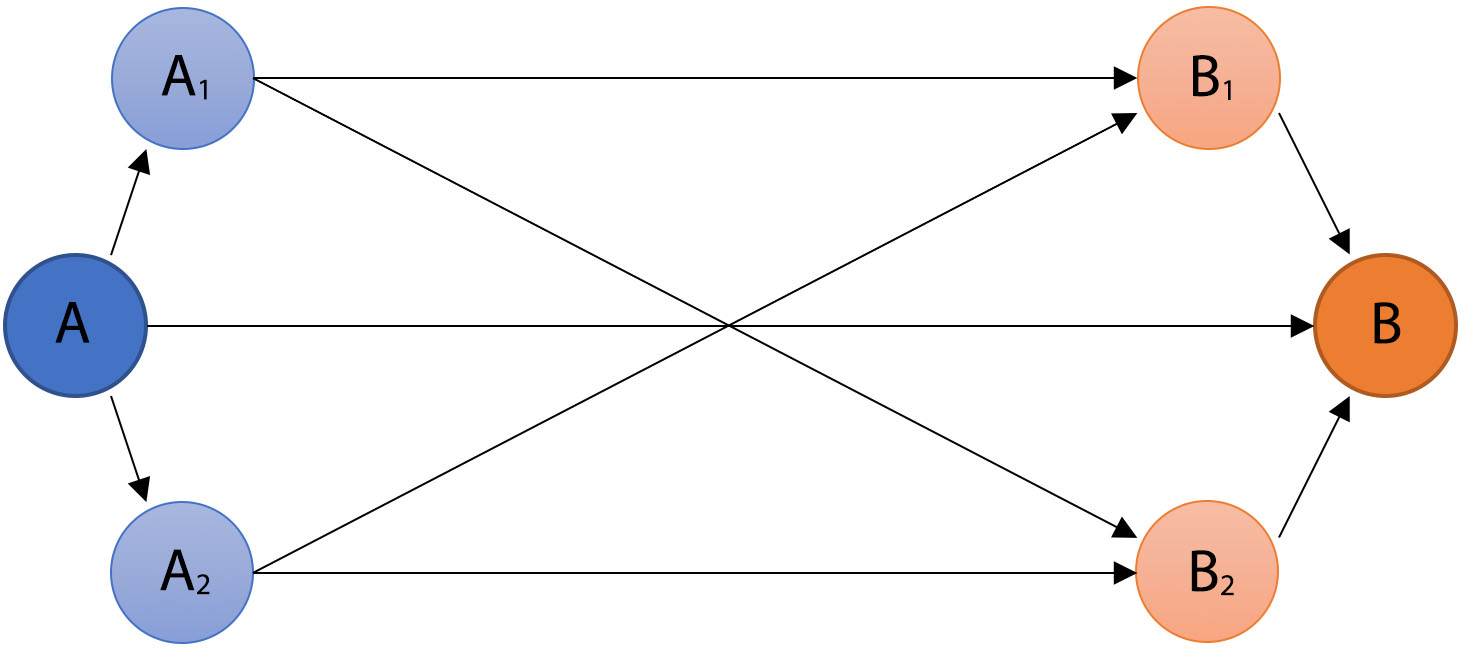
\includegraphics[width=0.8\textwidth]{Graph_example_n2}
  \label{fig:graph_example}
\end{figure}

\subsubsection{Driving Assumptions}

\FIXME{Add from pres}


\section{AI Concept : Search Strategies}\label{sec:search}

\subsection{Uniform Cost Search}

At the base line, our algorithm performs a tree search seeking to minimize the time it takes to travel given a price limit. 
Since different users may value their time more than their money or may not like driving, we considered the following features.

\FIXME{\subsubsection{Weight on Driving}}

\subsection{A* Search with Straight Line Heuristic}

In addition to the above features, we would like to improve upon our algorithm by adding a heuristic component to our cost function. 
Across edges, we are mixing different modes of transportation which have different speeds. Additionally, costs for flying depends only on plane tickets where as costs for driving depends directly on the distance and miles per gallon of a vehicle. 
For this reason, we can not simply just use the distance as a heuristic but we need to first convert it to the proper units based on what we would like to minimize.

\FIXME{\subsubsection{Estimating Price based on Distance} Prob won't get to...}

\subsubsection{Estimating Time based on Distance}



\FIXME{Alex - Commercial flights do not fly faster than 600 mph. So we could add (straight line distance)/600 to the path cost for time. This would favor contact points that are closer to the goal point.}

\section{Experimentation : Amite to Stockton}

To experiment with our algorithm we have chosen the example trip from Amite, LA to Stockton, CA. To see that our ai responds to minimizing different factors we compared the resulting solution sequences. 

\subsection{Uniform Cost Search}

In order to check that our program will consider the users price limit, we have done two searches. One without a price limit and one with a price limit of \$250.
\begin{center}
Solution : Amite $\rightarrow$ MSY(1.2 hr) $\rightarrow$ LAX1(4.4 hr) $\rightarrow$ Stockton(5.2 hr) \\
\quad Total Price: \$255 \\
\quad Total Time: 10 hrs and 48 min
\end{center}

\begin{figure}[!ht]
  %\caption{Search when minimizing time without price limit.}
  \centering
  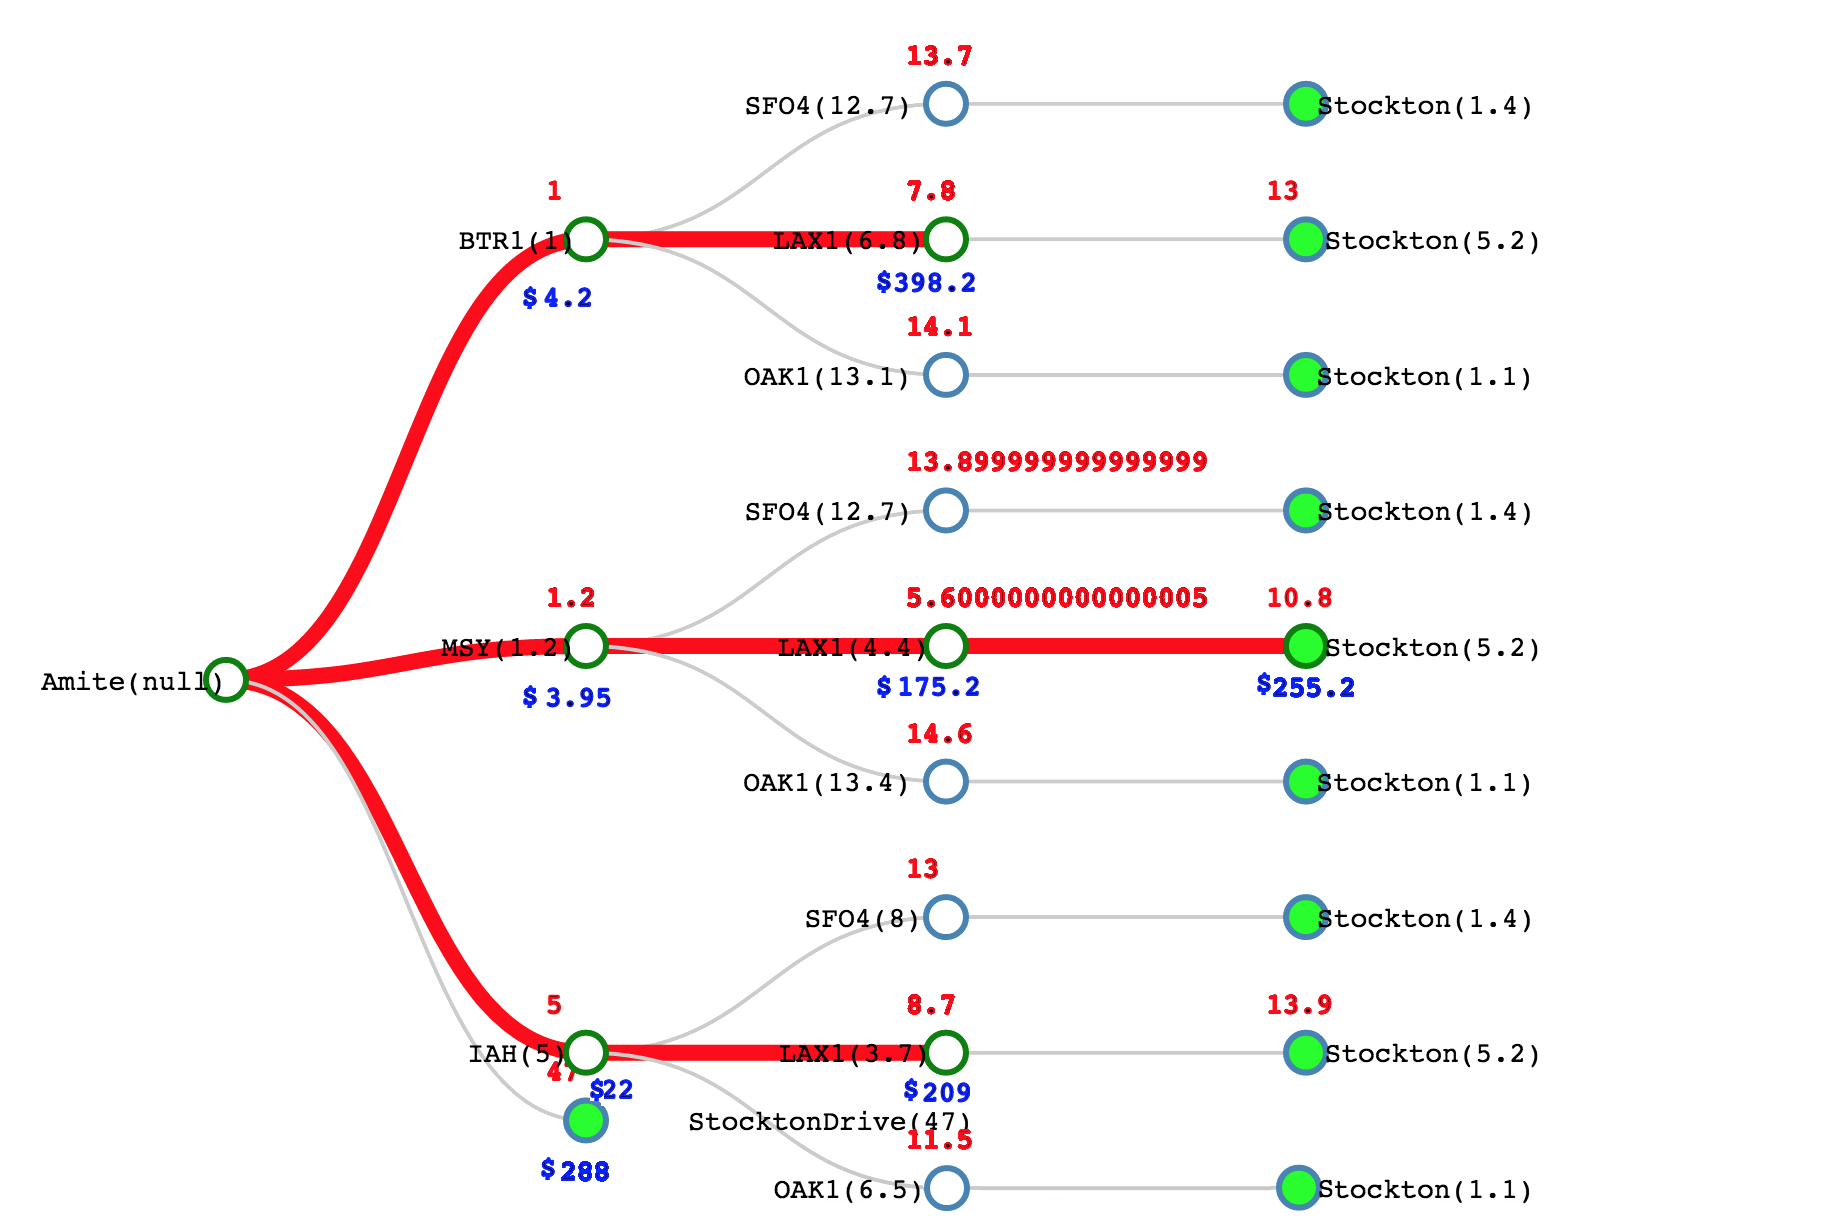
\includegraphics[width=0.8\textwidth]{time}
  \label{fig:time}
\end{figure}

\pagebreak

\begin{center}
Solution : Amite $\rightarrow$ IAH(5 hr) $\rightarrow$ LAX1(3.7) $\rightarrow$ Stockton(5.2) \\
\quad Total Price: \$230 \\
\quad Total Time: 13 hrs and 54 min\\
\end{center}

\begin{figure}[!ht]
  \centering
  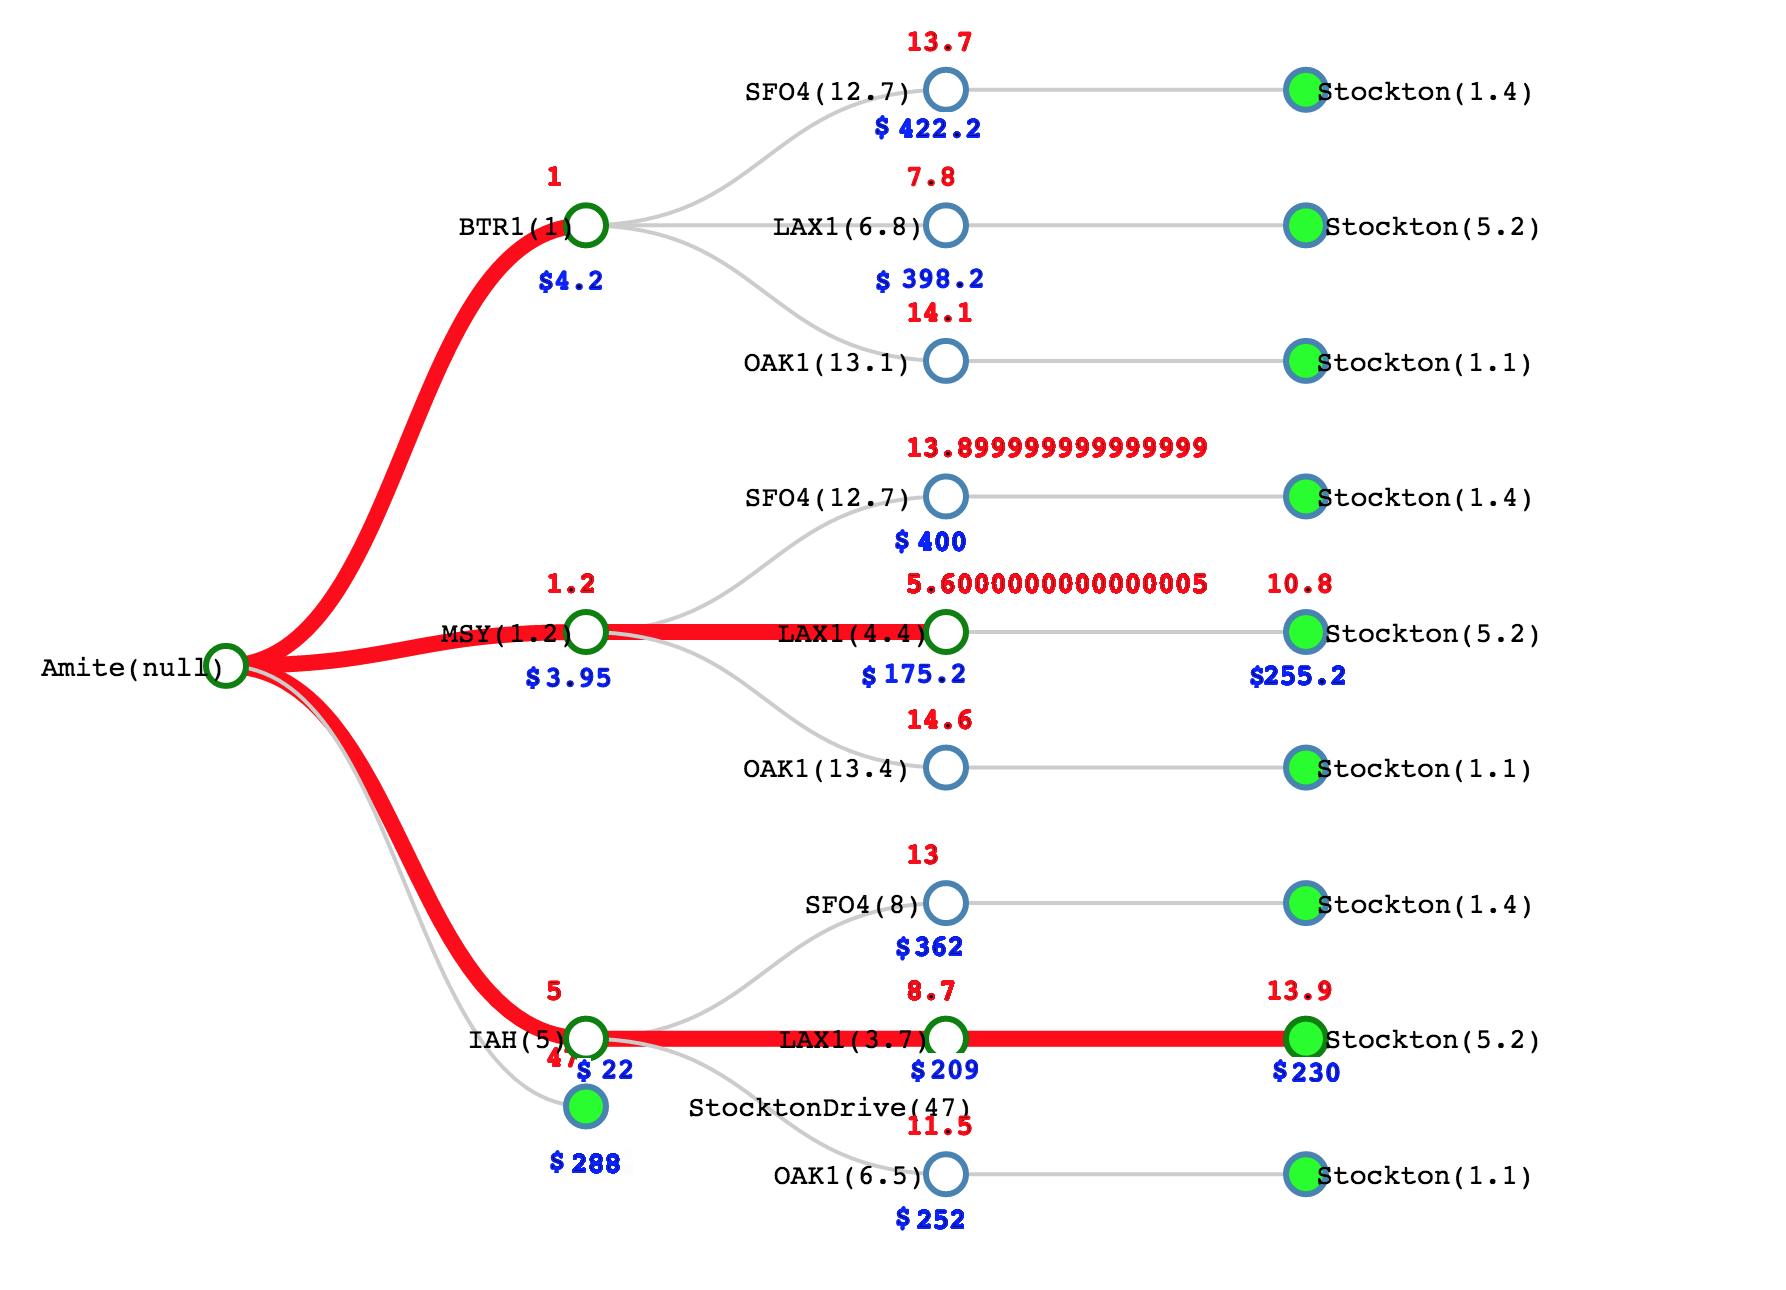
\includegraphics[width=0.8\textwidth]{time_lim}
  %\caption{Search when minimizing time with price limit of \$250.}
  \label{fig:time_lim}
\end{figure}

%\subsection{}

%\subsection{Conclusions}


\section{Software System Design and Implementation}
To compute the time and price of each edge we are using many different Google APIs.

\subsection{Object Oriented Design using Java}

\FIXME{UML Diagram from pres}

\subsection{APIs}

\FIXME{Explain what each do because Chet seemed interested.}
\begin{itemize}
\item QPX Express Airfare API
\item Google Maps Distance Matrix API
\item Google Maps Geocoding API
\item Google Maps Geolocation API
\item Google Maps Directions API
\item Google Places API Web Service
\end{itemize}

\subsection{Caching}
\FIXME{Even if we don't get this working we should still explain what we have with sqlite and what we wanted to do with bluemix and maybe even why we had trouble with it. A screenshot like the one from the pwrpt would be nice}

Some of the APIs are quite slow, especially the QPX Express Airfare API to find flights. 
We use two separate caches to make searches faster. One cache is used for road travel and one for flight. When we call the function used to determine the best route it first searches the cache to see if the query has already been made in the past. If it has, it returns the result of the query. If this data is not stored, the API is called and the resulting distance is stored in the cache. This speeds up searching significantly over time because the cache will be able to referenced more and more, avoiding calls to the API. The API calls take significantly longer than the cache calls, so it becomes faster and faster over time. 

\section{Future Work}
This application is restricted to traveling within the US. Other countries could be included to give the user the option to travel internationally. The only modes of transportation that are used are driving and flying. To give the user a more flexibility when traveling, other modes of transportation could be incorporated into this application such as walking, bicycling, taking the train or metro, and taking a ferry.

Additionally, after caching of a large amount of data our application could make certain predictions which improve our search algorithm.  For example, instead of choosing the $n$ nearest airports to add to our search tree, Watson Analytics predict feature could also choose an airport which may be slightly farther away but which may frequently have deals on flights.
				

\end{document}
